\section{Appendices}

\appendix

\section{Experiment Setup}
\label{app:setup}
\subsection{Datasets}
We evaluate the reasoning performance on three widely-used datasets: WebQSP~\citep{talmor2018web}, CWQ~\citep{talmor2018web}, and GrailQA~\citep{gu2021beyond}. These datasets are constructed based on Freebase and consist of natural language questions paired with their corresponding SPARQL queries. Specifically, WebQSP features questions where the topic entity and answer entities are at most 2 relation hops apart. CWQ extends WebQSP by incorporating more complex entities and constraints, with relation paths up to 4 hops. In contrast to WebQSP and CWQ, GrailQA is designed for a more comprehensive evaluation of generalization capabilities across three settings: independently and identically distributed (I.I.D.), compositional, and zero-shot.

To ensure consistent results and reduce evaluation overhead, we follow the setting of previous work~\citet{xiong2024interactive}, which uniformly sample questions across different types in WebQSP and CWQ. For the GrailQA dataset, we randomly sample 600 instances for evaluation.
\subsection{Baselines}
Our experiments compare \ours \space against two categories of methods.

\textbf{Fine-tuning-based Methods.} We consider two settings: fine-tuning on partial data (low-source setting) and on full data. In the low-source setting, we select the agentic approaches, includes the SFT model in Interactive-KBQA~\citep{xiong2024interactive}, which uses the same toolset as our method (abbreviated as SFT-traj.), two MCTS-based agentic methods, KBQA-o1~\citep{luokbqao1} and MCTS-KBQA~\citep{xiong2025mcts}. Notably, since our method is trained on only a subset of the data and uses no SPARQL annotations, its performance is directly comparable to this category of baselines.
For the full-data setting, which serves as a secondary point of reference, we include the SOTA SP-based methods RnG-KBQA~\citep{ye2022rng} and TIARA~\citep{shu2022tiara}.

\textbf{Prompting-based Methods.} We selected a diverse set of prompting strategies for comparison. These include methods based on direct prompting, Chain-of-Thought (CoT), and self-consistency with CoT; approaches that use an LLM to enhance semantic parsing (KB-BINDER\citep{li2023few} and KB-Coder~\citep{nie2024code}) and subgraph retrieval~\citep{tian2024augmenting}; and Interactive-KBQA~\citep{xiong2024interactive} that prompts an LLM to reason as an agent. For a fair comparison, we report the scores for these methods directly from their official papers, as the specific API versions used in their experiments are no longer accessible.

\subsection{Evaluation Metrics}
We primarily report the F1 score since the answers are returned as an unordered list. Following previous work~\citep{xiong2024interactive}, we also report Random Hits@1 (RHits@1) and Exact Match (EM) for reference. As our method is not fully based on semantic parsing, we do not report the semantically equivalent of logical forms (another score commonly abbreviated as EM) in ~\citet{gu2021beyond}.

\subsection{Implementation Details}
We use the Qwen2.5-Coder-7B-Base as our backbone LLM. For the cold-start stage, our implementation is based on the LlamaFactory framework~\citep{zheng2024llamafactory}; we use a cosine learning rate schedule with an initial learning rate of 2e-5, a batch size of 8, and a maximum sequence length of 4096. We fine-tune the model for 8 epochs. In the RL stage, our implementation is based on Agent-R1 framework \citep{Agent-R1} (a verl-based \citep{sheng2024hybridflow} agentic training framework); we set the number of rollouts to N=8, use a batch size of 64 for rollout, and a global batch size 512 for training. We train the model for 1 epoch. At validation, we set the temperature to 0 to ensure deterministic outputs. The detail parameters can be found in \ref{tab:base_settings}. All experiments were conducted on 8 $\times$ NVIDIA H100 (80GB) GPUs and 8 $\times$ NVIDIA A100 (80GB) GPUs.

\begin{table}[htbp]
\centering
\caption{Key parameters during the training process.}
\label{tab:base_settings}
\begin{tabular}{lc}
\toprule
\textbf{Parameter} & \textbf{Value} \\
\midrule
SFT settings \\
\midrule
Batch size  & 8 \\
Learning Rate & 2e-5 \\
Max Response Length & 4096 \\
Algorithm & LoRA \\
Epoch & 8 \\
\midrule
RL settings \\
\midrule
Rollout Batch Size & 64 \\
Rollout N & 8 \\
Global-batch Size & 512 \\
Learning Rate & 1e-6 \\
Learning Rate Warmup Steps & -1(disabled) \\
Max Prompt Length & 4096 \\
Max Response Length & 8192 \\
KL Loss Coefficient & 0.001 \\
Algorithm & GRPO \\
Epoch & 1\\
Validation Temperature & 0.0 \\
Rollout Temperature & 1.0 \\
\bottomrule
\end{tabular}
\end{table}
\section{Further Analysis}
In this section, we provide several supplementary analyses. First, we examine the impact of different backbone models on performance and discuss our method's token efficiency. These results justify our model selection and highlight the efficiency advantages of our approach. Second, we present a joint distribution of error frequency versus sample accuracy across training stages, which serves to supplement our main analysis of training dynamics (Section~\ref{sec:trian_dym}) and offers a more comprehensive view of how the agent's capabilities evolve.
\subsection{Analysis of the Impact of Different Backbones}
We compared the impact of different backbone models on performance during the cold-start stage. As shown in Table~\ref{tab:model_performance}, our results indicate that Qwen2.5-Coder-7B-Base delivers the strongest overall performance. Although Qwen3-8B-Base performs better on the simpler WebQSP dataset, we selected Qwen2.5-Coder-7-Base for its superior performance on CWQ, which contains more complex questions. Furthermore, our task involves numerous code-style tool calls, where a coder-specialized model has a natural advantage. 
\begin{table}
  \centering
  \caption{Performance comparison of various backbone models across three benchmark datasets.}
  \label{tab:model_performance}
  \begin{tabular}{lcccccc}
    \toprule
    \multirow{2}{*}{\textbf{Model}} & \multicolumn{2}{c}{\textbf{WebQSP}} & \multicolumn{2}{c}{\textbf{CWQ}} & \multicolumn{2}{c}{\textbf{GrailQA}} \\
    \cmidrule(lr){2-3} \cmidrule(lr){4-5} \cmidrule(lr){6-7}
    & F1   & Hits@1 & F1   & EM   & F1   & EM   \\
    \midrule
    Qwen2.5-Coder-3B-Base & 58.4 & 63.9 & 36.7 & 41.2 & 58.4 & 68.2 \\
    Qwen2.5-Coder-7B-Base & 56.7 & 64.9 & 50.5 & 59.8 & 63.1 & 68.4 \\
    Qwen3-4B-Base    & 63.9 & 69.4 & 38.4 & 39.0 & 55.0 & 59.1 \\
    Qwen3-8B-Base    & 65.3 & 71.6 & 44.6 & 45.8 & 60.1 & 63.1 \\
    \bottomrule
  \end{tabular}
\end{table}
\subsection{Analysis of token efficiency}
To evaluate the inference efficiency of our method, we conducted a computational cost analysis against prompting-based baselines, including the single-round inference method CoT and the multi-round interactive method ToG. As shown in Table~\ref{tab:cost_hit}, the comparison covers LLM call frequency, token usage, and overall cost. The results reveal that \ours \space achieves performance comparable to the complex ToG, while maintaining a computational budget similar to the much simpler CoT. This efficiency stems from outcome-based supervision: the model learns to recover from empty results or intermediate errors in a single pass, obviating the need to generate multiple branches to find a solution at significant computational expense. Overall, \ours \space shifts the efficiency frontier toward lower cost while maintaining strong effectiveness, making it more predictable and easier to deploy in real-world scenarios.
\begin{table}[ht]
  \centering
  \small
  \caption{Cost and effectiveness on CWQ and WebQSP.}
  \label{tab:cost_hit}

  % -------- CWQ --------
  \begin{tabular}{lcccc}
    \toprule
    \multicolumn{5}{c}{\textit{CWQ}} \\
    \midrule
    Model & \# Avg. LLM Call & Total Token & Total Cost & Hit@1 \\
    \midrule
    CoT  & 1.0 & 409.7   & \(8.00\times10^{-5}\) & 43.7 \\
    ToG  & 9.2 & 11468.5 & \(2.30\times10^{-3}\) & 69.5 \\
    Ours & \underline{5.0} & \underline{660.6} & \textbf{\(0\)} & \textbf{75.7} \\
    \bottomrule
  \end{tabular}

  % -------- WebQSP --------
  \begin{tabular}{lcccc}
    \toprule
    \multicolumn{5}{c}{\textit{WebQSP}} \\
    \midrule
    Model & \# Avg. LLM Call & Total Token & Total Cost & Hit@1 \\
    \midrule
    CoT  & 1.0 & 397.6   & \(8.00\times10^{-5}\) & 47.5 \\
    ToG  & 8.8 & 10189.4 & \(2.10\times10^{-3}\) & 82.6 \\
    Ours & \underline{3.9} & \underline{439.6} & \textbf{\(0\)} & \underline{80.1} \\
    \bottomrule
  \end{tabular}
\end{table}
\subsection{Analysis on Overall Robustness Capability Shift}
To further investigate how the agent's robustness evolves, we analyze the association between intermediate errors and final rewards throughout training. As illustrated in Figure~\ref{fig:union_dynamic}, we plot the joint distribution of the mean frequency of empty results/errors per question against the mean reward. This visualization reveals a clear progression. Early in training, the distribution forms a downward-sloping triangle, where higher error rates are strongly correlated with lower rewards. As training advances, this shape flattens into a rectangle, indicating that high rewards are achieved even with a non-trivial frequency of errors. Concurrently, the density increases in the upper-left corner, reflecting a growing number of questions being solved directly and perfectly. The transformation provides compelling evidence of our method's superiority: the agent not only learns to avoid mistakes but also develops the crucial ability to recover from them, transitioning from a brittle execution policy to a robust, high-scoring one.

\begin{figure}[!t]
    \centering
    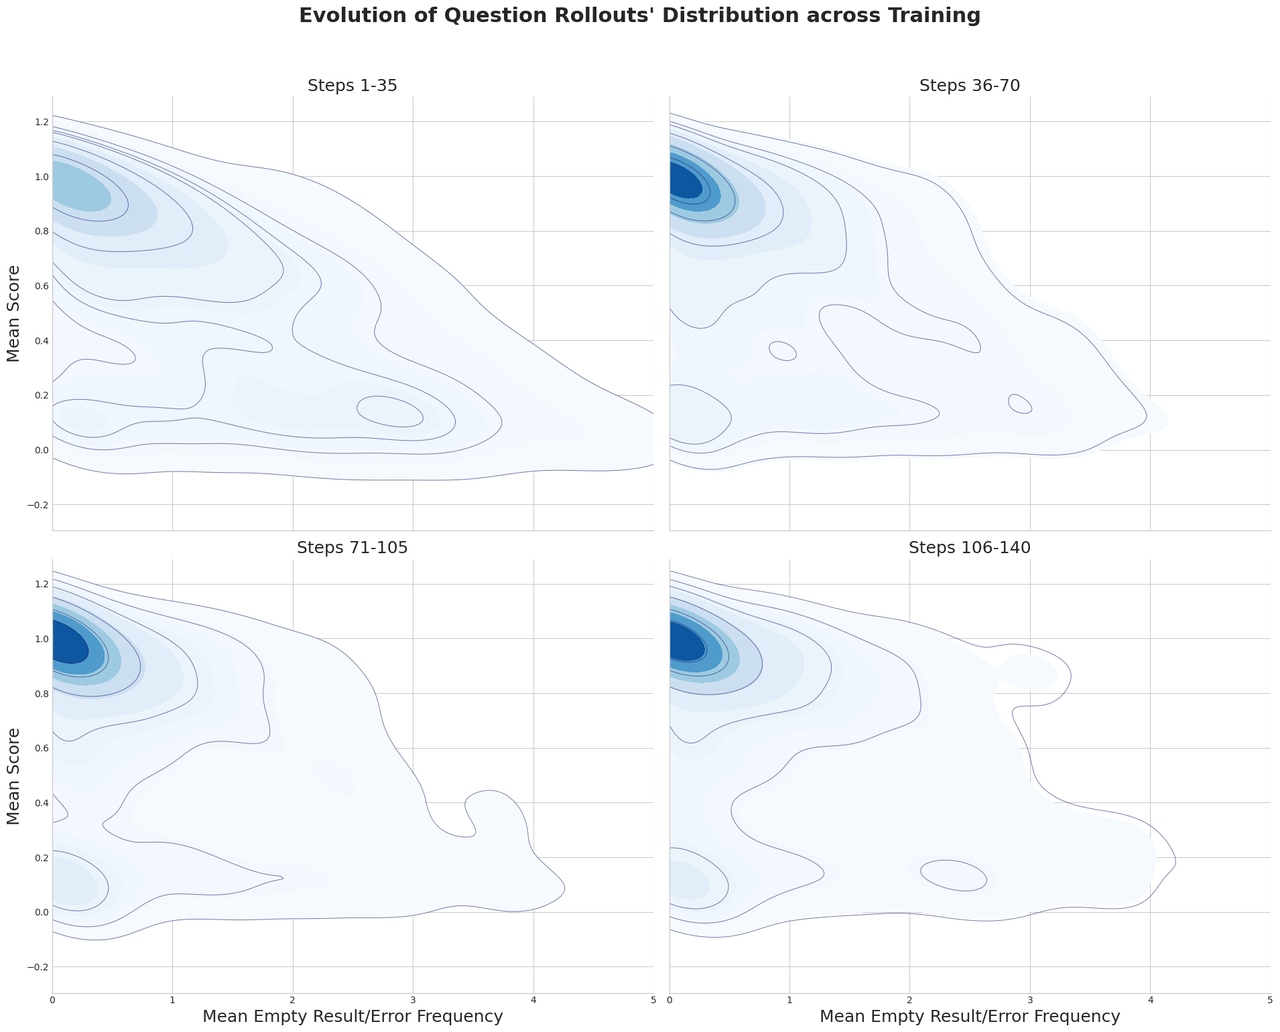
\includegraphics[width=0.9\linewidth]{figures/union_dynamic.png}
    \caption{Joint distribution of mean empty-result/error frequency and mean reward across training phases.}
    \label{fig:union_dynamic}
\end{figure}
\section{Statistics}
\label{app:stat}
We give the statistic of training samples used in cold-start-stage and RL stage on three datasets. 
\begin{table}[h]
\centering
\caption{Number of samples for different training stages across the WebQSP, CWQ, and GrailQA datasets.}
\label{tab:training_samples}
\begin{tabular}{l ccc}
\toprule
\textbf{Stage} & \textbf{WebQSP} & \textbf{CWQ} & \textbf{GrailQA} \\
\midrule
RL-Phase-1  & 1265 & 2400 & 1800 \\
RL-Phase-2  & 709  & 1600 & 1200 \\
Cold-Start & 440  & 699  & 563  \\
\bottomrule
\end{tabular}
\end{table}

\section{Error Analysis}
\label{app:error}
\begin{figure*}[!t]
    \centering
    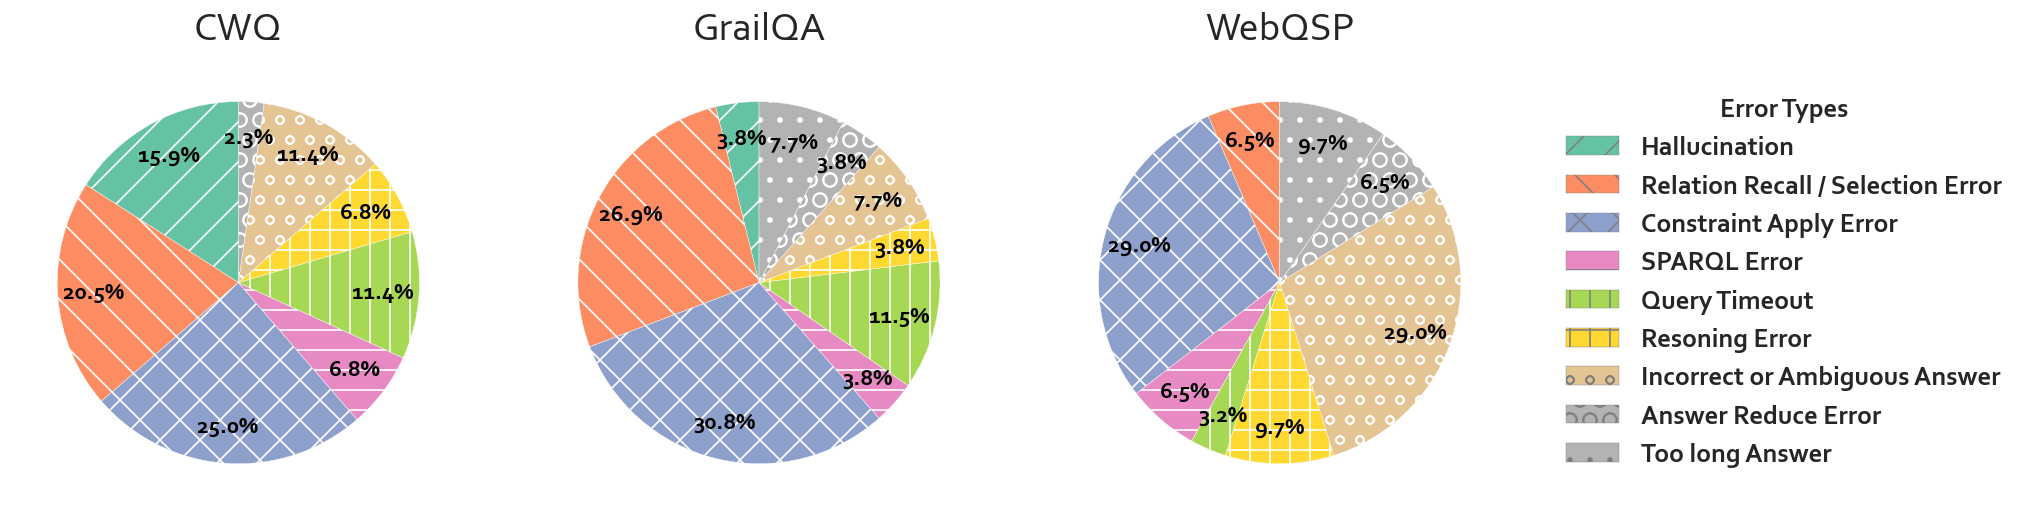
\includegraphics[width=1\linewidth]{figures/error.png}
    \caption{Analysis of sampled failure cases per dataset. We visualize the proportion of factors contributing to errors.}
    \label{fig:error}
\end{figure*}
To identify the limitations of our method, we conducted an error analysis by manually inspecting random sampled cases where the $F_1$ score was less than 1. The results are categorized in Fig.~\ref{fig:error}, with the primary error types being Hallucination, Constraint Application Error, and Relation Recall/Selection Error. Hallucinations often result from flawed self-correction attempts. While intuitively detrimental, our prior experiments show that penalizing such behavior actually stifles the model's capacity for self-correction. The other two error types generally stem from incorrect decisions during complex reasoning. These errors highlight the space for future work: enhancing the model's ability to handle complex questions within a linear decision-making process. Notably, the high rate of constraint errors on WebQSP is due to the model failing to identify implicit temporal constraints (e.g., the KB's 2015 cutoff date) in present-tense questions.
\section{Prompts}
\label{app:prompt}


In our experiments, the same prompt was used for both training and evaluation, which is composed of a system prompt and a user prompt.
\begin{examplebox}{System Prompt}
\begin{lstlisting}
#Tools

You are an expert in knowledge base query language SPARQL programming. The user gives a question, and you need to iteratively call the tool to continuously improve the SPARQL query until it can get the answer to the question.

You are provided with function signatures within <tools></tools> XML tags:
<tools>
{'type': 'function', 'function': {'name': 'SearchGraphPatterns', 'description': 'This tool searches for relevant one-hop and two-hop subgraphs tied to a specified variable. It queries subgraphs where the chosen variable (?x, assuming the SPARQL query begins with "SELECT DISTINCT ?x WHERE") appears as the head or tail entity and returns them collectively. The semantic parameter indicates the expected predicate semantics. When provided, the tool ranks the subgraphs based on these semantics. If unspecified, it returns the complete subgraph.', 'parameters': {'type': 'object', 'properties': {'sparql': {'type': 'string', 'description': 'SPARQL query'}, 'semantic': {'type': 'string', 'description': 'The semantic parameter represents the expected predicate semantics.'}}, 'required': ['sparql']}}}

{'type': 'function', 'function': {'name': 'ExecuteSPARQL', 'description': 'This tool executes a SPARQL query and returns the results.', 'parameters': {'type': 'object', 'properties': {'sparql': {'type': 'string', 'description': 'SPARQL query'}}, 'required': ['sparql']}}}

{'type': 'function', 'function': {'name': 'SearchTypes', 'description': 'Search the knowledge base for matching semantic types, used to initiate queries from a type when no topic entities are available, or to find a type to refine the query when multiple entities are returned. When use the type, please give the sparql as: SELECT DISTINCT ?x WHERE { ?x ns:type.object.type ns:<type_name> }', 'parameters': {'type': 'object', 'properties': {'query': {'type': 'string', 'description': 'the semantic of type to search for'}}, 'required': ['query']}}}
</tools>

For each function call, return a json object with function name and arguments within <tool_call></tool_call> XML tags:
<tool_call>
{{"name": <function-name>, "arguments": <args-json-object>}}
</tool_call>
\end{lstlisting}
\end{examplebox}

\begin{examplebox}{User Prompt}
\begin{lstlisting}
When you encounter a complex question, you should break it down into several sub-questions and answer them step by step. You can use the tools provided. You can use the tool as many times as you want.
You must first conduct reasoning inside <think>...</think>. If you need to use the tool, you can use the tool call <tool_call>...</tool_call> to call the tool after <think>...</think>.
When you have the final answer, you can output the answer in the python list format inside <answer> tag, such as: <answer> the answer is \\boxed{{[...]}} </answer>.

Output format for tool call:
<think>
...
</think>
<tool_call>
...
</tool_call>

Output format for answer:
<think>
...
</think>
<answer>
...
</answer>

Question: {question}
Topic Entities: {topic entities}
Assistant:
\end{lstlisting}
\end{examplebox}
\section{Case Study}
\label{app:case}
To illustrate the flexibility and robustness of our agent's reasoning process, we present two representative case studies. The first case demonstrates robustness: when faced with two consecutive empty query results, the agent successfully recovers by leveraging a more distant observation from its history to try a new, promising relation, ultimately finding the correct answer. The second case highlights flexibility and self-correction, showing the agent's ability to identify an illogical query result (e.g., receiving a high school when a university was expected) and adapt its strategy by employing a novel action to resolve the issue.

\begin{table*}
  \caption{Example of robust reasoning of \ours.}
  \label{tab:case-study-1}
  \begin{center}
  % \newcolumntype{L}{>{\raggedright\arraybackslash}X}
  \begin{tabularx}{\textwidth}{ L }
  \toprule
  \textbf{Question:} who plays london tipton in suite life on deck? \\
  \midrule
  \thinkrow{I need to find the actor who plays London Tipton in "The Suite Life on Deck". I will start by searching for predicates related to "actor" or "performance" for the entity "London Tipton(m.07g8r3)".}
  \searchrow{SearchGraphPatterns(sparql="SELECT ?e WHERE \{ VALUES ?e \{ns:m.07g8r3\} \}", semantic="actor/performer")}
  \resultrow{[..., (?e, film.film\_character.portrayed\_in\_films -> film.performance.actor, "Brenda Song"),...]}
  \thinkrow{(Fail Try 1)...}
  \searchrow{ExecuteSPARQL(sparql="SELECT ?actor WHERE \{ VALUES ?e1 \{ns:m.07g8r3\} . VALUES ?e2 \{ns:m.03mj4jm\} . ?e1 ns:film.film\_character.portrayed\_in\_films ?cvt . ?cvt ns:film.performance.actor ?actor . ?cvt ns:film.performance.film ?e2 . \}")}
  \resultrow{[]}
  \thinkrow{\textbf{The previous query returned no results. This might be due to the structure of the predicates or the way the entities are linked. I will try a different approach by searching for predicates related to "actor" or "performance"}...}
  \searchrow{SearchGraphPatterns(sparql="SELECT ?e WHERE \{ VALUES ?e \{ns:m.03mj4jm\} \}", semantic="actor/performer/character")}
  \resultrow{[...,(?e, award.award\_nominated\_work.award\_nominations -> award.award\_nomination.award, "Kids' Choice Award for Favorite TV Actor"), ...]}
  \thinkrow{(Fail Try 2)...}
  \searchrow{ExecuteSPARQL(sparql="SELECT ?actor WHERE \{ VALUES ?e1 \{ns:m.07g8r3\} . VALUES ?e2 \{ns:m.03mj4jm\} . ?e2 ns:award.award\_nominated\_work.award\_nominations ?cvt . ?cvt ns:award.award\_nomination.award\_nominee ?actor . ?cvt ns:award.award\_nomination.character ?e1 . \}")}
  \resultrow{[]}
  \thinkrow{\textbf{The previous queries have not yielded the correct result. I need to refine my approach.} The question asks for... I will try a different strategy...I will try to find the actor who played London Tipton in any film and then filter for "The Suite Life on Deck".}
  \searchrow{ExecuteSPARQL(sparql="SELECT ?actor WHERE \{ VALUES ?e \{ns:m.07g8r3\} . ?e ns:film.film\_character.portrayed\_in\_films ?cvt . ?cvt ns:film.performance.actor ?actor . \}")}
  \resultrow{["Brenda Song"]}
  \answerrow{Brenda Song} 
  \bottomrule
  \end{tabularx}
  \end{center}
\end{table*}

\begin{table*}[!t]
  \caption{Example of flexible reasoning of \ours.}
  \label{tab:case-study-2}
  \begin{center}
   \begin{tabularx}{\textwidth}{ L }
  \toprule
  \textbf{Question:} Where did Charles Drew attend \textbf{college} that has the latest founding date? \\
  \midrule
  \thinkrow{I need to find the colleges that Charles R. Drew attended and then find the college with the latest founding date.}
  % \searchrow{SearchGraphPatterns(sparql="SELECT ?e WHERE \{ VALUES ?e \{ns:m.018t67\} \}", semantic="attended college")}
  % \resultrow{[...(?e, people.person.education -> education.education.institution, "Dunbar High School"), ...]}
  % \thinkrow{The `SearchGraphPatterns` results for "attended college" show that `people.person.education -> education.education.institution` is the predicate pair. I will use this predicate pair to find the colleges attended by Charles R. Drew. Then, for each college, I will need to find its founding date to determine which one has the latest founding date.}
  % \searchrow{SearchGraphPatterns(sparql="SELECT ?college WHERE \{ VALUES ?e \{ns:m.018t67\} . ?e ns:people.person.education ?edu . ?edu ns:education.education.institution ?college . \}", semantic="founding date")}
  % \resultrow{[...(?college, organization.organization.date\_founded, "1754")...]}
  % \thinkrow{The `SearchGraphPatterns` results for "founding date" show that `organization.organization.date\_founded` is the predicate for the founding date... I will find the colleges attended by Charles R. Drew and their founding dates, then order by founding date in descending order and limit to 1 to get the college with the latest founding date.}
  (Omit for space...)
  \\
  \searchrow{ExecuteSPARQL(sparql="SELECT DISTINCT ?college WHERE \{ VALUES ?e \{ns:m.018t67\} . ?e ns:people.person.education ?edu . ?edu ns:education.education.institution ?college . ?college ns:organization.organization.date\_founded ?founded\_date . \} ORDER BY DESC(xsd:date(?founded\_date)) LIMIT 1")}
  \resultrow{["Dunbar High School"]}
  \thinkrow{\textbf{The result is "Dunbar High School", but the question asks for the college, not high school. I need to re-evaluate the search.} ... I will search for the type "College/University".}
  % \searchrow{SearchGraphPatterns(sparql="SELECT ?e WHERE \{ VALUES ?e \{ns:m.018t67\} \}", semantic="attended educational institution")}
  % \resultrow{[...]}
  % \thinkrow{The `SearchGraphPatterns` results for "attended educational institution" show that...I will filter these institutions to include only those of type "College/University". I will search for the type "College/University".}
  \searchrow{SearchTypes(query="College/University")}
  \resultrow{["education.university", ...]}
  \thinkrow{The "SearchTypes" results include "education.university" ... I will find the colleges attended by Charles R. Drew and their founding dates, then order by founding date in descending order and limit to 1 to get the college with the latest founding date.}
  \searchrow{ExecuteSPARQL(sparql="SELECT DISTINCT ?college WHERE \{ VALUES ?e \{ns:m.018t67\} . ?e ns:people.person.education ?edu . ?edu ns:education.education.institution ?college . ?college ns:type.object.type ns:education.university . ?college ns:organization.organization.date\_founded ?founded\_date . \} ORDER BY DESC(xsd:date(?founded\_date)) LIMIT 1")}
  \resultrow{["McGill University Faculty of Medicine"]}
  \answerrow{McGill University Faculty of Medicine} 
  \bottomrule
  \end{tabularx}
  \end{center}
\end{table*}
